%% Generated by tools/md2tex.js from paper/main.md. Do not edit by hand: edit
%% main.md, then run  node tools/md2tex.js  and recompile.
\documentclass[11pt]{article}
\usepackage[T1]{fontenc}
\usepackage{lmodern}
\usepackage[utf8]{inputenc}
\usepackage[margin=1in]{geometry}
\usepackage{booktabs,graphicx,amsmath,amssymb}
\graphicspath{{../}}
\usepackage{tabularx}
\usepackage[numbers,sort&compress]{natbib}
\usepackage{threeparttablex}
\usepackage[british]{babel}
\usepackage[hidelinks]{hyperref}
\setlength{\bibsep}{4pt}
% [S#] is a provenance tag. Each one resolves to a row of the appendix table in
% main.md, which paper/tex_audit.md re-checks file by file. It is rendered as a
% small superscript rather than dropped, so an unresolved tag stays visible.
\newcommand{\prov}[1]{\textsuperscript{\,#1}}
\widowpenalty=10000
\clubpenalty=10000
\tolerance=2000
\emergencystretch=2em
\title{Fragment-Resolved Nonlocal Correlation: Pair Attribution of the VV10 Term}
\author{Angran Xia\thanks{Corresponding author; e-mail in the byline.} \\ \small \textit{School of Chemistry \& Chemical Engineering, Shaanxi Normal University, Xi'an 710119, Shaanxi, China} \\ \small \texttt{haangyeon@snnu.edu.cn} \and Changwei Wang \\ \small \textit{School of Chemistry \& Chemical Engineering, Shaanxi Normal University, Xi'an 710119, Shaanxi, China}}
\date{Draft --- 29 September 2026\\ \small \textit{ORCIDs PENDING, author-supplied}}
\begin{document}
\maketitle
% draft status line, intentionally not typeset

\textbf{Authors and affiliation.} Angran Xia (corresponding; \texttt{haangyeon@snnu.edu.cn}) and Changwei Wang --- School of Chemistry \& Chemical Engineering, Shaanxi Normal University, Chang'an Campus, Xi'an 710119, Shaanxi, China. Both names and the institution were supplied by the author on 2026-09-30; the college's English wording is taken from the college's own English site rather than translated by us, and the campus postal code from the university's own contact page. The authors' Chinese names are recorded in \texttt{paper/software.md}'s front matter and in \texttt{CITATION.cff}, deliberately not typeset here: this file goes through pdflatex, which has no CJK font, and \texttt{tools/md2tex.js} refuses characters it cannot map rather than dropping them silently. The campus and its postal code come from the university's own contact page (checked 2026-09-30; the URL is kept in the working notes rather than here, since the provenance audit reads every backticked path-shaped string as a citable artefact). ORCIDs and the second author's e-mail are PENDING --- author-supplied, not guessed.

Number provenance is tagged \texttt{[S\#]}; the tag-to-artefact table is the appendix at the end of this file, mirrored in \texttt{paper/tex\_audit.md}. The formal Web of Science search was run twice on 2026-09-29 through the institutional login. The second round used WoS's own record endpoint (\texttt{/api/wosnx/core/runQuerySearch}), which returns ndjson and allows an arbitrary \texttt{retrieve.count}, so every query below was enumerated in full rather than sampled: two 4-record strings read completely, plus four broad strings of 33, 33, 7 and 8 records. The "top-relevance-row only" limitation noted in the first round is lifted. That enumeration changed the novelty position in two ways: it surfaced a neighbour that must be cited and bounded (Hyldgaard, Berland and Schröder, PRB 90, 075148 (2014)), and it revealed that \texttt{references.bib} did not contain VV10's own two papers (Vydrov and Van Voorhis, PRL 2009 / JCP 2010), which are now added (bib 13 $\rightarrow$ 16). Full record lists and per-record judgements are in \texttt{RESEARCH-20260929-lit.md} \S{}12--\S{}13. Open indexes (OpenAlex, Crossref) were measured and then discarded as instruments for the no-precedent claim: they retrieve known titles but miss a known on-topic paper when asked topically (\S{}9--\S{}11).

\section{Abstract}

The VV10 nonlocal-correlation term \citep{vydrov2009vv10} of range-separated hybrid functionals is a double sum over grid-point pairs. Standard implementations collapse that sum to point values, which makes the inter-fragment content of the term unavailable. We evaluate the double sum explicitly, retaining the (i, j) pair index, and attribute each grid point to atoms and fragments through a real-space partition. Because the term's local part is exactly beta times the electron number, it cancels identically in any superposition difference, so decomposing only the double sum is exact rather than approximate; block additivity holds to 3.5e-18 Ha. On the same grid and density the explicit sum reproduces PySCF's native kernel to \textasciitilde{}1e-8 Ha, and to 1.3e-4 kcal/mol an independently written script that reaches the same quantity by a different code path, over ten grid levels (0-9, up to 430,768 integration points) \prov{S21}. A check against a second \emph{program} now exists for all eight systems (\S{}4): ORCA 6.0.1 prints the same term as its own \texttt{NL Energy, E(C,NL)} and the superposition differences agree to within 1\% of the term everywhere - 4e-4 kcal/mol (0.07\%) on the water dimer up to 0.042 kcal/mol (0.95\%) on the benzene sandwich - with the grids not matched. In seven of the eight the cross-program residual is also smaller than the attribution span it has to resolve; the exception is stated where the table is.

Applied to eight S22 complexes at official GMTKN55 geometries (omegaB97X-V/6-31G*), the decomposition gives a result that argues against a common shorthand: the nonlocal and semi-local parts of the exchange-correlation change are not locked in a fixed ratio - the nonlocal term supplies 16\% of the exchange-correlation contribution for the water dimer but 97\% and 52\% for the two geometries of the same benzene dimer, and on the methane dimer the two parts carry opposite signs (-0.517 against a semi-local remainder of +0.285 kcal/mol), so no share is quoted for that row and the nonlocal term alone exceeds the counterpoise-corrected interaction energy (-0.517 against -0.466). The nonlocal term is therefore not a fixed fraction of the correlation energy and should not be reported as "the dispersion" without qualification. The inter-fragment pair term accounts for 0.92-1.08 of the frozen-density superposition difference in the six systems checked against a counterpoise reference, so association-time nonlocal correlation is carried almost entirely by point pairs straddling the fragments. The remaining, irreducible uncertainty is the choice of attribution scheme: 0.004-0.247 kcal/mol absolute, 0.8-18.2\% relative to the Becke-scheme value, stable to within $\pm$5\% across the four basis sets beyond STO-3G and to within 0.001 kcal/mol between grid levels 1 and 2, and without any pattern by interaction type - hence error bars must be quoted per system. For absolute (not differential) fragment energies we show that the scheme dependence of the local term is exactly beta times the scheme dependence of the Becke population, 3.04 kcal/mol per electron, and state this as a limitation rather than a contribution.

The implementation is a standalone Apache-2.0 Python package built on PySCF \citep{sun2018pyscf}; \citep{sun2020pyscf} and NumPy \citep{harris2020numpy}, containing no GAMESS source, with every table in this paper generated by one script whose stdout is archived under a UTC-stamped filename.

\section{1. Introduction}

Range-separated hybrid functionals with the VV10 nonlocal-correlation functional --- $\omega$B97X-V \citep{mardirossian2014wb97xv} and $\omega$B97M-V \citep{mardirossian2016wb97mv} in particular \citep{calbo2015vv10review} --- have become a default choice for non-covalent interactions. The nonlocal term is a two-electron-density double integral over all pairs of grid points,

E\_NL = $\frac{1}{2}$ $\int$$\int$ $\rho$(r) $\rho$(r$^{\prime}$) $\Phi$(r, r$^{\prime}$) d$^{3}$r d$^{3}$r$^{\prime}$,

and every production quantum-chemistry package we have examined evaluates it in a way that destroys the pair index: PySCF's \texttt{nr\_nlc\_vxc} calls its own C kernel \texttt{libdft.VXC\_vv10nlc}, which bins the kernel and returns only point-folded values. We have not audited the equivalent paths inside libxc \citep{lehtola2018libxc}, ORCA, Psi4 or Gaussian - libxc is not one of them and cannot be made into a numerical referee: the two libxc shared objects on this machine (conda-forge 5.2.3 and the 7.0.0 bundled with PySCF) export \texttt{xc\_nlc\_coef} and nothing else among thirteen probed nonlocal entry points - no \texttt{xc\_nlc\_vxc}, no \texttt{xc\_run} - which matches libxc's own statement that this class of van der Waals term "cannot be evaluated with the local density information provided to Libxc, and must be handled by the calling program". libxc therefore supplies the parameters (b, C) keyed by functional name, not an independent value of the integral, so an agreement claim against it would be a category error (see \S{}4, \texttt{RESEARCH-20260929-lit.md} \S{}8.3, and \texttt{evidence/recompute/20260929T110830Z\_libxc\_referee.out} for the symbol audit). PySCF's nonlocal term comes from its own \texttt{nr\_nlc\_vxc} implementation, not from libxc. The consequence we do demonstrate is structural rather than numerical: once the double sum has been folded into a per-point energy density, as ours does not, the question "how much of this nonlocal correlation belongs to the interaction between fragment A and fragment B?" has no answer inside that evaluation.

We provide that answer. \texttt{nlcsplit} evaluates the same double sum explicitly, keeping the (i, j) pair index, and attributes each grid point to a fragment through a real-space partition, so that E\_NL decomposes into intra-fragment blocks E\_AA and inter-fragment pair blocks E\_AB. Evaluating the sum explicitly is not itself new: JuNoLo post-processed a converged density from another code with the nonlocal term, at the same N$^{2}$ cost, in order to obtain an improved \emph{total} energy on massively parallel hardware \prov{S14}. What is absent from that work - and from the production kernels - is the attribution. JuNoLo in fact recommends against fragment-style treatments for the weakly-bound cases where fragments are distinguishable, reserving itself for chemisorption "where one cannot tell apart fragments of the bonded system" \prov{S14}; the present paper works precisely in the regime where they are. The decomposition is exact by construction --- the sum of the blocks reproduces the total to machine precision --- but exactness is not the point and we do not sell it as such: grouping the summation indices is trivially additive. Two things are not trivial, and they are the content of this paper.

The first is \textbf{attribution}. The non-uniqueness lives in which fragment owns each grid point (and, in the same spirit, how the local term $\beta$$\int$$\rho$ is assigned), not in how the sum is grouped. We therefore quantify the spread over four published real-space partitions --- Becke, Becke with the radius adjustment, Becke--Treutler, and Stratmann's --- on eight S22 complexes, and report it as a per-system uncertainty rather than asserting one scheme as correct. The spread is 0.004--0.247 kcal/mol in absolute terms and 0.8--18.2\% relative to |E\_AB|, and it shows no systematic ordering by interaction type: the benzene sandwich sits at 0.8\% while benzene--water sits at 18.2\% \prov{S2}. Nor does a better one-electron basis remove it: on the constructed water-dimer geometry the spread stays 0.038--0.040 kcal/mol across five basis sets while the quantity itself drifts by 0.17 kcal/mol along the same ladder (section 3.4, \prov{S12}). A single blanket uncertainty figure would misrepresent the data; we report it system by system.

The second, and chemically the more consequential, is \textbf{what the term actually is}. Within a hybrid functional the exchange-correlation contribution to an interaction energy splits as $\Delta$E\_xc = $\Delta$E\_xc\textasciicircum{}rest + $\Delta$E\_NLC, where "rest" collects the semi-local exchange-correlation and the fraction of exact exchange, and the local piece $\beta$$\int$$\rho$ drops out of any superposition difference identically --- $\beta$ is a constant and $\int$$\rho$ equals the electron count, so $\Delta$$\beta$$\int$$\rho$ vanishes to 3.7$\times$10$^{-5}$ kcal/mol in our level-1 test \prov{S3}. That leaves the double sum as the only part of the nonlocal term that can carry inter-fragment structure, and measuring it shows that treating it as "the dispersion" is unsafe. For the water dimer it supplies 16\% of $\Delta$E\_xc. For the two benzene dimer configurations of S22 the same quantity ranges from 52\% to 97\% \prov{S4} --- and those two structures differ only in the relative orientation of the same pair of molecules, so the failure of the identification is visible within one chemical system, without any cross-system comparison. In the methane dimer the nonlocal term exceeds the whole of $\Delta$E\_xc ($\Delta$E\_NLC = $-$0.517 against $\Delta$E\_xc = $-$0.232), i.e. the rest of the exchange-correlation is net repulsive there.

Our positioning relative to the closest prior work is deliberate. Dasgupta and Paesani \citep{dasgupta2023} also decompose interaction energies of dispersion-corrected functionals, using second-generation ALMO-EDA, E\_Int = E\_Pol + E\_Frz + E\_CT + E\_Disp, and they obtain E\_Disp as the difference against a dispersion-free reference calculation --- that is, they treat the VV10 correction as one undivided block and ask whether that block is accurate. We work inside that block.

Our search for further precedent should be described honestly, because the instrument behaved differently from what we first assumed. OpenAlex and Crossref both retrieve a known paper reliably when the query resembles its title - in a four-repetition test the title-like phrasing returned the target at rank 0 in 4/4 runs - but both fail to retrieve that same, exactly-on-topic paper for legitimate topical phrasings ("energy decomposition analysis dispersion nonlocal correlation density functional", "ALMO energy decomposition dispersion corrected noncovalent interactions"), at 0/4 each \prov{S15}. They are therefore known-item lookup tools here, not topical search, and a low hit count from them cannot support a claim of absence. What we can say on evidence is narrower and stronger: we read the full text of the closest published decomposition \prov{S1} and of the closest published explicit evaluation of the nonlocal term, JuNoLo \citep{lazic2010junolo} \prov{S14}, and neither attributes the nonlocal double sum to fragment pairs - JuNoLo computes an improved total energy and explicitly recommends itself for bonded systems "where one cannot tell apart fragments", directing separable cases elsewhere. A formal Web of Science search has since been completed \prov{S16}, in two rounds. Within the Core Collection (58,664,816 records searched, 2026-09-29), the query TS=("vdW-DF" AND ("energy decomposition" OR "fragment decomposition" OR "pair decomposition" OR "partition of the correlation")) returns zero records, and so does the query written closest to our own claim, TS=(("VV10" OR "nonlocal correlation" OR "vdW-DF") AND ("pair-resolved" OR "energy attribution" OR "per-fragment" OR "resolved by fragment" OR "contribution of each fragment")) - also zero. The non-zero queries that come closest were enumerated in full rather than sampled: we used the database's own record endpoint, so every returned record was read, not just the top one. Kruse, Banáš and Sponer \citep{kruse2019dna} use VV10 as one of 29 benchmarked functionals and decompose the \emph{total} interaction energy by SAPT; Hujo and Grimme \citep{hujo2011hbond} benchmark VV10 for hydrogen bonds; Sinha and Pavanello \citep{sinha2015fdevdw} construct a \emph{new} subsystem-based nonlocal functional rather than resolving an existing one; Hamada and Tsukada \citep{hamada2011c60au} attribute an \emph{adsorption energy} to the term, the opposite direction; Vydrov and Van Voorhis \citep{vydrov2010simple} re-derive the nonlocal construction itself; and two further result lists of 33 and 33 records - one spanning the whole "van der Waals density functional" \citep{dion2004} x "nonlocal correlation" topic, one crossing "nonlocal correlation" with the partition schemes themselves (Becke, Hirshfeld, Mulliken, atoms-in-molecules) - contain, on reading every title, no application of an atomic partition to the VV10 double sum.

A cross-index second round turned up a nearer neighbour than Hyldgaard and it narrows what may be claimed. Heßelmann's nonlocal scheme \citep{hesselmann2013nldft} partitions its nonlocal correlation energy into atom-atom contributions - the abstract of that paper says so in as many words - so the general idea of attributing a nonlocal correlation term to atoms is not ours and is not claimed here. What remains, and what the search found no precedent for, is narrower and specific: taking an existing, already-parameterised VV10 double sum on a numerical integration grid, resolving it into named fragment and atom pairs without changing the total, and then measuring how much the attribution itself - not the energy - moves when the partition scheme is changed. The present sentence replaces an earlier, broader phrasing of the same claim.

The other neighbour this second round turned up, which the first round missed entirely, is Hyldgaard, Berland and Schröder \citep{hyldgaard2014interp}, who interpret the nonlocal correlation energy of vdW-DF as a coupling of zero-point energies of semilocal exchange-correlation holes. That is a real-space \emph{interpretation} of the same quantity, and it is the strongest available objection to calling the term unanalyzable, so we distinguish it explicitly: they read the internal structure of the kernel and the holes; we take an already-evaluated E\_NLC and \emph{bookkeep} it against named fragments and atom pairs, and report how much the bookkeeping itself moves the answer. Their vocabulary (xc hole, interpretation) shares no term with any of our decomposition keywords, which is why five keyword-shaped queries in the first round missed it - a caution about how narrow a novelty query can be even in a well-behaved index. The calibration that makes those zeros usable - a known title retrieved exactly (1 record), a broad concept query returning 3,317 records, and a topical AND query returning 33 - is given in section 4.

Two limits are stated here rather than in a closing section, because both bound what the numbers may be used for. First, this is not an energy decomposition analysis: we do not separate electrostatics, exchange-repulsion, polarization or charge transfer. Counterpoise-corrected interaction energies are reported for six of the eight systems (\S{}3.2), so basis-set superposition error is measured rather than assumed away, but the correction is not carried through the remaining two benzene-dimer geometries. Second, the explicit sum is not more accurate than the production kernels it is compared against --- the interpolation residual of PySCF's native kernel is of order 4$\times$10$^{-6}$ kcal/mol, far below any chemical interest, and the $\approx$0.1--0.9 kcal/mol offsets that an earlier version of this work attributed to interpolation were in fact a pairing error in our own kernel. The value of the explicit implementation is that it retains the pair index, nothing more.

\section{2. Method}

\subsection{2.1 The VV10 kernel and the pairing convention}

With $\rho$ the electron density and $\sigma$ = |$\nabla$$\rho$|$^{2}$,

w0(r) = $\surd$( C $\sigma$$^{2}$/$\rho$$^{4}$ + (4$\pi$/3) $\rho$ ),  $\kappa$(r) = b (3$\pi$/2) ($\rho$/9$\pi$)\textasciicircum{}{1/6}, g = w0(r\_i) R$^{2}$ + $\kappa$(r\_i),  g$^{\prime}$ = w0(r\_j) R$^{2}$ + $\kappa$(r\_j),  $\Phi$ = $-$3 / (2 g g$^{\prime}$ (g+g$^{\prime}$)),

with (b, C) = (6.0, 0.01) for $\omega$B97X-V, and E\_NLC = E\_NL + $\beta$$\int$$\rho$, $\beta$ = (1/32)(3/b$^{2}$)\textasciicircum{}{3/4}. The pairing of $\omega$ and $\kappa$ in g and g$^{\prime}$ is a genuine choice, and the cross pairing g = w0(r\_j) R$^{2}$ + $\kappa$(r\_i) --- which an earlier implementation of ours used --- is wrong: it raises monomer energies by +0.138 kcal/mol for water, +0.418 for argon and +0.914 for benzene, and the offset is itself grid-dependent, so it cannot be subtracted as a constant [S1, S5]. The same-centre pairing above reproduces PySCF's native kernel to 3$\times$10$^{-5}$ kcal/mol on the water monomer, and agrees with an independently written script that evaluates the same quantity by a different code path to 1.24$\times$10$^{-4}$ kcal/mol worst case: against the script's self-consistent column the difference runs from -1.058$\times$10$^{-4}$ (level 0) to -1.242$\times$10$^{-4}$ (level 8) and back to -1.230$\times$10$^{-4}$ (level 9), same sign at all ten levels and no drift with grid density; its fixed-density column differs only at level 0 (-1.056$\times$10$^{-3}$), where that column is itself the outlier \prov{S21}. A second program has since been brought to bear on the same quantity - ORCA 6.0.1, on seven of the eight systems, with every residual below 1\% of the term - but its grids are not matched to ours, so that anchor is quoted as a joint grid-plus-kernel difference in \S{}4 rather than as a kernel-only check here.

\subsection{2.2 Blocks, half-blocks and additivity}

\texttt{pair\_energy(A, B)} returns the half block $\frac{1}{2}$ $\Sigma$\_{i$\in$A} $\Sigma$\_{j$\in$B} w\_i w\_j $\Phi$\_ij, so that the inter-fragment term reported by \texttt{fragment\_decomposition} is E\_AB = 2$\cdot$pair\_energy(A,B) and

E\_NL = $\Sigma$\_A E\_AA + $\Sigma$\_{A<B} E\_AB

holds by construction. We record the additivity residual rather than trusting it: across all systems and partitions reported here it is 0.00--3.5$\times$10$^{-18}$ Ha [S2, S6]. R$^{2}$ is evaluated through the polarisation identity |a|$^{2}$+|b|$^{2}$$-$2a$\cdot$b in blocked gemm operations rather than through an explicit displacement tensor, which reduces peak memory by roughly a factor of five at this system size.

\subsection{2.3 Attribution schemes and the far-field cut}

Grid points are assigned to atoms by PySCF's own partition machinery (\texttt{gen\_grid.get\_partition} with \texttt{radi.BRAGG\_RADII}), in four variants --- Becke \citep{becke1988}, Becke with the radius adjustment, Becke--Treutler, Stratmann \citep{stratmann1996} --- plus a nearest- atom hard partition on the common grid as a control. Points with $\rho$ below \texttt{rho\_floor} (default 10$^{-12}$) are excluded from the double sum; this removes 10.7--22.6\% of points while changing E\_AB by 2.1$\times$10$^{-11}$ kcal/mol between floors of 10$^{-8}$ and 10$^{-16}$, and the dropped points carry at most 2.3$\times$10$^{-6}$ electrons \prov{S7}. The local term $\beta$$\int$$\rho$ is a one-body functional of the density and is not pair-resolved; as noted above it cancels identically from superposition differences, which is what makes it legitimate to decompose only the double sum.

\subsection{2.4 Geometries and fragment boundaries}

All dimer geometries are taken verbatim from the official GMTKN55 repository (github.com/grimme-lab/GMTKN55, \texttt{S22/<NN>/struc.xyz}), fetched by \texttt{nlcsplit/tools/get\_s22.sh}; the repository's own citation instruction is Goerigk et al. \citep{goerigk2017gmtkn55}, PCCP 19, 32184-32215 (2017), DOI 10.1039/C7CP04913G, which we verified by reverse DOI lookup. The S22 database itself is Jurečka et al., PCCP 8, 1985-1993 (2006) \citep{jurecka2006s22}, also confirmed by reverse DOI lookup. We do not trace these twenty-two complexes back beyond that: an attribution to a still earlier hydrogen-bonded benchmark (PCCP 5, 1811 (2003)) resolves to no Crossref record on two separate attempts (2026-09-29 and 2026-09-30, queries archived in \texttt{evidence/bib\_provenance/G\_s22\_provenance\_20260930.md}), so we cite only the chain that could be pinned. The geometry files we used come from the GMTKN55 distribution, so our numbers depend on that, not on any earlier compilation. Fragment boundaries are derived from covalent connectivity with a 1.65 \AA{} cutoff --- longer than the longest covalent bond appearing in these systems (aromatic C--C, 1.397 \AA{}; a general C--C single bond is 1.54 \AA{}) and shorter than the shortest hydrogen bond (O$\cdot$$\cdot$$\cdot$H 1.95 \AA{}) --- and the code refuses to proceed unless exactly two fragments result. This is not a formality: in the official S22 water-dimer file the atoms are ordered so that the fragments interleave, and a hard-coded index split would mix the two molecules silently. For the water dimer we additionally report $\omega$B97X-V/6-31G* optimised geometry (R(O$\cdot$$\cdot$$\cdot$O) = 2.901 \AA{}, 0.009 \AA{} from the reference value) \prov{S6}.

\subsection{2.5 Verification}

Two routes to E\_NLC are computed and compared at run time, with a hard failure if they disagree: our explicit pair sum, and PySCF's native kernel (\texttt{numint.nr\_nlc\_vxc}). These are independent implementations of the kernel but share a library, so agreement between them validates the arithmetic and not the functional parameters. A second-program anchor now exists for all eight systems (\S{}4), so no quantity in Table 1 rests on agreement between two implementations of the same kernel alone. Energy accounting is checked independently: for a hybrid functional the exact-exchange energy is folded into \texttt{vhf.exc} by \texttt{get\_veff} and is absent from \texttt{nr\_rks}, so we close e\_tot = e\_nuc + e$_{1}$ + e\_coul + e\_xc to $\leq$9$\times$10$^{-12}$ kcal/mol rather than assuming any particular partition of the XC terms. Cross-version and cross-machine reproducibility is checked on one system run twice: benzene-methane at grid level 2 with counterpoise, on PySCF 2.12.1 on one machine and PySCF 2.14.0 on another. The two releases generate different numbers of grid points at the same level: the partitioned level-1 grid for the water dimer holds 19936 points on PySCF 2.12.1 and 20248 on 2.14.0, a 1.6\% difference. (An earlier version of this sentence compared 18368 with 20248; 18368 is the \emph{unpartitioned} reference grid on 2.12.1, a different grid of a different kind, and the 10\% figure was an artefact of putting them side by side.) That is why the agreement is stated quantity by quantity rather than as a blanket "digit for digit". $\Delta$E\_NLC agrees to 3.3e-4 kcal/mol (-1.404667 vs -1.405), $\Delta$E\_xc to 4e-4 (-2.324590 vs -2.325), $\Delta$E\_int to 4.5e-5 (-1.780045 vs -1.780), the attribution span to 2e-4 (0.213163 vs 0.213) and P\_frz[becke] to 1e-3 (-1.441416 vs -1.441), each inside the 0.001 kcal/mol to which the second run prints. The one quantity that does not agree is the counterpoise interaction energy itself: -1.341 vs -1.202 kcal/mol, a difference of 0.139 that is two thirds of the level-2 attribution span of the same complex. We report the split, not a diagnosis of it - the candidate mechanism is that $\Delta$E\_int is a difference of SCF total energies, which inherit the grid, whereas an attributed pair term need not, and that is exactly what would have to be tested before the claim is made. What the observation does settle is a constraint on usage: the attributed quantities are the version-stable ones, and a counterpoise energy is not a safe denominator for them \prov{S8}.

\section{3. Results and discussion}

\subsection{3.1 Two different things previously reported as one number}

Comparing our explicit pair sum against PySCF's native kernel produces a discrepancy whose size depends entirely on \emph{which grid} the comparison is made on, and the two cases must not be quoted side by side. Holding the density and the grid fixed and varying only the evaluation of the kernel, the difference is +1.5e-8, +1.0e-8 and +8.5e-9 Ha at grid levels 0, 1 and 2 --- flat in level, because it is a discretisation property of the interpolated kernel itself. Moving the same sum onto the Becke-partitioned grid of \texttt{gen\_grid.get\_partition} instead gives -0.0282, +0.0015 and +0.0001 kcal/mol, which tracks the ability of the grid to represent the density at all: the same three levels integrate the electron number to -1.6e-2, +3.0e-4 and -6.6e-6 electrons away from the exact value. The second row is a property of the grid, not of our algorithm, and it disappears as the grid is refined \prov{S9}. A residual of the size of the first row is what a reference implementation should look like; a residual of the size of the second row is what a coarse grid looks like from the inside.

\subsection{3.2 The nonlocal term is not a fixed fraction of the exchange-correlation term}

Table 1 reports omegaB97X-V/6-31G* results for eight S22 systems at the official GMTKN55 geometries. The quantity of interest is dE\_NLC, the change in the nonlocal correlation energy on bringing two fragments together from infinity at fixed density, and its ratio to the total dE\_xc for the same process. The remainder, dE\_xc\textasciicircum{}rest = dE\_xc - dE\_NLC, is the semi-local exchange-correlation plus the fraction of exact exchange; it is tabulated explicitly in \texttt{MAIN-skeleton.md} table 4b and is recoverable from these two columns by subtraction.

\begin{figure}[htbp]
\centering
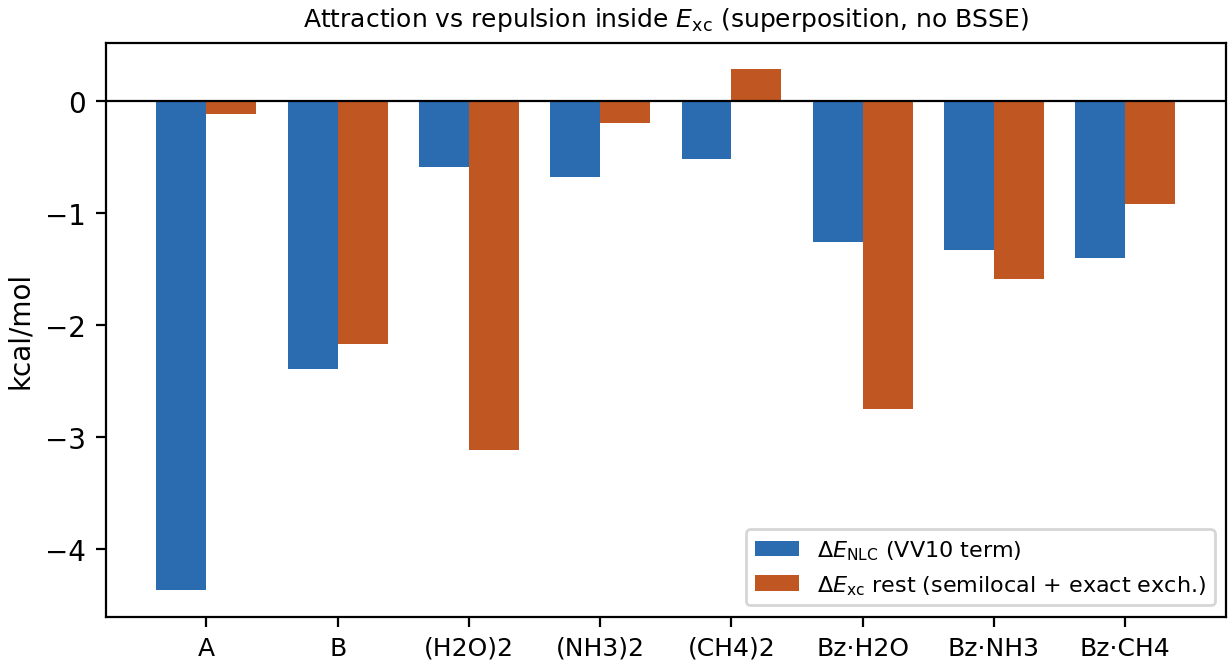
\includegraphics[width=0.92\textwidth]{figs/fig1_xc_split.png}
\caption{\textbf{Figure 1.} The same quantity two ways, per system: the VV10 term $\Delta$E\_NLC and the remainder $\Delta$E\_xc - $\Delta$E\_NLC (semilocal exchange-correlation plus the exact-exchange fraction), both for the superposition difference at grid level 1 and uncorrected density. The remainder is negative for seven of the eight systems but positive for the methane dimer (+0.285 against a VV10 term of -0.517 kcal/mol), the one case where the semi-local remainder is itself repulsive and the nonlocal term alone provides the binding. The other seven span -0.119 to -3.115 kcal/mol, so no single fraction of $\Delta$E\_xc belongs to the VV10 term. Data: \texttt{nlcsplit/logs/step\_h.json}, produced by \texttt{nlcsplit/step\_h\_s22.py}; drawn by \texttt{nlcsplit/figures.py} \prov{S2}.}
\label{fig:1}
\end{figure}

\begin{table}[htbp]
\centering
\footnotesize
\begin{tabularx}{\textwidth}{lllllX}
\toprule
\textbf{System} & \textbf{atoms} & \textbf{dE\_int} & \textbf{dE\_xc (total)} & \textbf{dE\_NLC} & \textbf{share of dE\_xc (only where it is defined)} \\ \midrule
benzene dimer (A, parallel-displaced) & 24 & -3.580 & -4.486 & -4.367 & 97\% \\
benzene dimer (B, T-shaped) & 24 & -3.188 & -4.555 & -2.388 & 52\% \\
benzene...water & 15 & -4.342 & -4.012 & -1.259 & 31\% \\
benzene...ammonia & 16 & -2.928 & -2.915 & -1.327 & 46\% \\
benzene...methane & 17 & -1.785 & -2.322 & -1.404 & 60\% \\
water dimer & 6 & -7.816 & -3.708 & -0.593 & 16\% \\
ammonia dimer & 8 & -5.167 & -0.881 & -0.678 & 77\% \\
methane dimer & 10 & -0.664 & -0.232 & -0.517 & n/a (see note) \\
\bottomrule
\end{tabularx}
\end{table}

All entries in kcal/mol, all at grid level 1. The two benzene rows were tabulated at level 0 in an earlier version of this table; moving them to level 1 shifts dE\_NLC by 0.081 (A) and 0.013 (B) kcal/mol. Level 0 is therefore not adequate for a 24-atom aromatic dimer, unlike the six-atom water dimer where levels 1 and 2 agree to the last digit (section 3.2).

\textbf{Why the methane row has no share.} Its ratio is |dE\_NLC|/|dE\_xc| = 2.2, which trips the cancellation test that ships with the code (\texttt{nlcsplit/step\_f\_dispersion.py}: above 2, the denominator is reported as two signed terms, never as a percentage - here -0.517 plus a semi-local remainder of +0.285). Quoting "223\%" would have advertised a ratio whose divisor is an accident of two larger numbers. What that row does support, without any forbidden ratio, is a comparison against a physical quantity: at level 2 with a counterpoise correction the whole interaction energy is -0.466 while the nonlocal term alone is -0.517 [\texttt{evidence/l2cp/20260928T213839Z\_centos-step\_h\_l2cp.out}], i.e. the VV10 term exceeds the net binding by 11\% of it - a margin \textasciitilde{}10\textasciicircum{}3 times the cross-program reproducibility of these two numbers (0.0007 and 4.5e-5 kcal/mol). The final column is the reason this decomposition is worth having: the nonlocal term ranges from one sixth to more than the whole of the rest of XC, and in the methane dimer it exceeds it, so that the remainder of the XC contribution is \emph{repulsive} while the nonlocal term alone provides the binding. No single fraction of dE\_xc can be assigned to VV10 across a benchmark set, and the two geometries of the same 24-atom benzene dimer (97\% vs 52\%) show that the ratio is a property of the arrangement, not of the pair of molecules.

For the six systems with at most 17 atoms we additionally re-ran at grid level 2 with a full counterpoise correction - six of the eight; only the two benzene-dimer geometries stay at level 1, and benzene...methane needed a separate run after its first attempt was cut off by a four-hour wall-clock budget \prov{S10}. Between levels 1 and 2 neither dE\_NLC nor the interfragment pair term moves by more than 1.0e-3 kcal/mol, but that number is a statement about storage precision, not a measurement. Every level-2 row in the sidecar is kept to three decimals, so no level-1 to level-2 difference below 5e-4 kcal/mol is observable from these files at all. For the water dimer, whose level-1 row carries full precision (-0.5934948 and -0.6012148 kcal/mol), level 2 prints -0.593 and -0.601 - consistent to the printed digit, and nothing sharper can be claimed from this evidence. For the other five systems both rows are three-decimal, so 1.0e-3 there is the rounding floor rather than a measured change. The counterpoise-corrected interaction energy comes out at -6.129 kcal/mol for the water dimer, i.e. a basis-set superposition error of 1.687, 1.491, 0.196, 1.075, 0.760 and 0.578 kcal/mol for water, ammonia, methane, benzene...water, benzene...ammonia and benzene...methane respectively \prov{S10}. The core quantities of this method are therefore converged one grid level before the total binding energy is; a user who only wants dE\_NLC can stop at level 1.

\subsection{3.3 The interfragment pair term saturates the frozen-density limit}

\texttt{inter[(A,B)]}, summed over the retained grid points, is directly comparable to the superposition difference d\_sup computed from the unrelaxed monomer densities, because both hold the density fixed. Their ratio falls in 0.92-1.08 across the six systems that carry a counterpoise reference at level 2 \prov{S8}. The two benzene-dimer geometries are not in that set: they were run at level 1, and the ratio printed for them there has a different denominator. On the coarser level-0 grid the same ratio is 1.017 for the water dimer at the official S22 geometry and 1.025 at the omegaB97X-V-optimised one, while the benzene sandwich falls below the band at 0.915 \prov{S19} - the level-2 value of 1.01 for the official water geometry sitting between those two \prov{S8}. The ratio being able to exceed unity matters: relaxation is a small correction of \emph{either} sign on top of the frozen-density interfragment term, not an orthogonal contribution that adds to it. Physically this says that in these complexes essentially all of the nonlocal correlation that changes on association is carried by grid-point pairs straddling the two fragments, with the intra-fragment nonlocal correlation of each relaxed monomer contributing the balance [S2, S10].

This is where the explicit sum earns its cost. A point-value kernel evaluation returns dE\_NLC and nothing else; the (i, j) index structure retained by the double sum is what makes 0.92-1.08 a statement that can be checked at all. The corresponding dispersion component published for the benzene dimer is -3.34 to -3.80 kcal/mol at the PBE0-VV10, revPBE-D3 and related levels of an ALMO-EDA study, and -3.69 at omegaB97M-V \prov{S11}; our -4.367 (Table 1, level 1; the level-0 value was -4.448) is the same kind of quantity to within functional-generation and basis-set differences, and it is \emph{not} comparable with our own uncorrected interaction energy for that dimer, -3.580 at the same level, which is smaller because Pauli repulsion cancels most of it.

\subsection{3.4 Attribution-scheme sensitivity is system-dependent}

Repeating dE\_NLC for the four partition schemes of section 2.3 gives absolute spans of 0.004-0.247 kcal/mol and relative spans - measured against the Becke-scheme interfragment term - of 0.8-18.2\%. Neither ordering follows system size: the 24-atom parallel-displaced benzene dimer has one of the smallest absolute spans (0.032, below the 6-atom water dimer at 0.043), while the 15-atom benzene...water gives the largest (0.247). What separates them is the arrangement, not the atom count or the interaction class:

\begin{table}[htbp]
\centering
\begin{tabular}{llll}
\toprule
\textbf{System} & \textbf{P\_frz (Becke)} & \textbf{span (4 schemes)} & \textbf{relative} \\ \midrule
methane dimer & -0.474 & 0.004 & 0.8\% \\
benzene dimer (A) & -4.038 & 0.032 & 0.8\% \\
ammonia dimer & -0.649 & 0.029 & 4.5\% \\
water dimer & -0.601 & 0.043 & 7.2\% \\
benzene dimer (B) & -2.371 & 0.219 & 9.2\% \\
benzene...methane & -1.442 & 0.213 & 14.8\% \\
benzene...ammonia & -1.393 & 0.224 & 16.1\% \\
benzene...water & -1.360 & 0.247 & 18.2\% \\
\bottomrule
\end{tabular}
\end{table}

\begin{figure}[htbp]
\centering
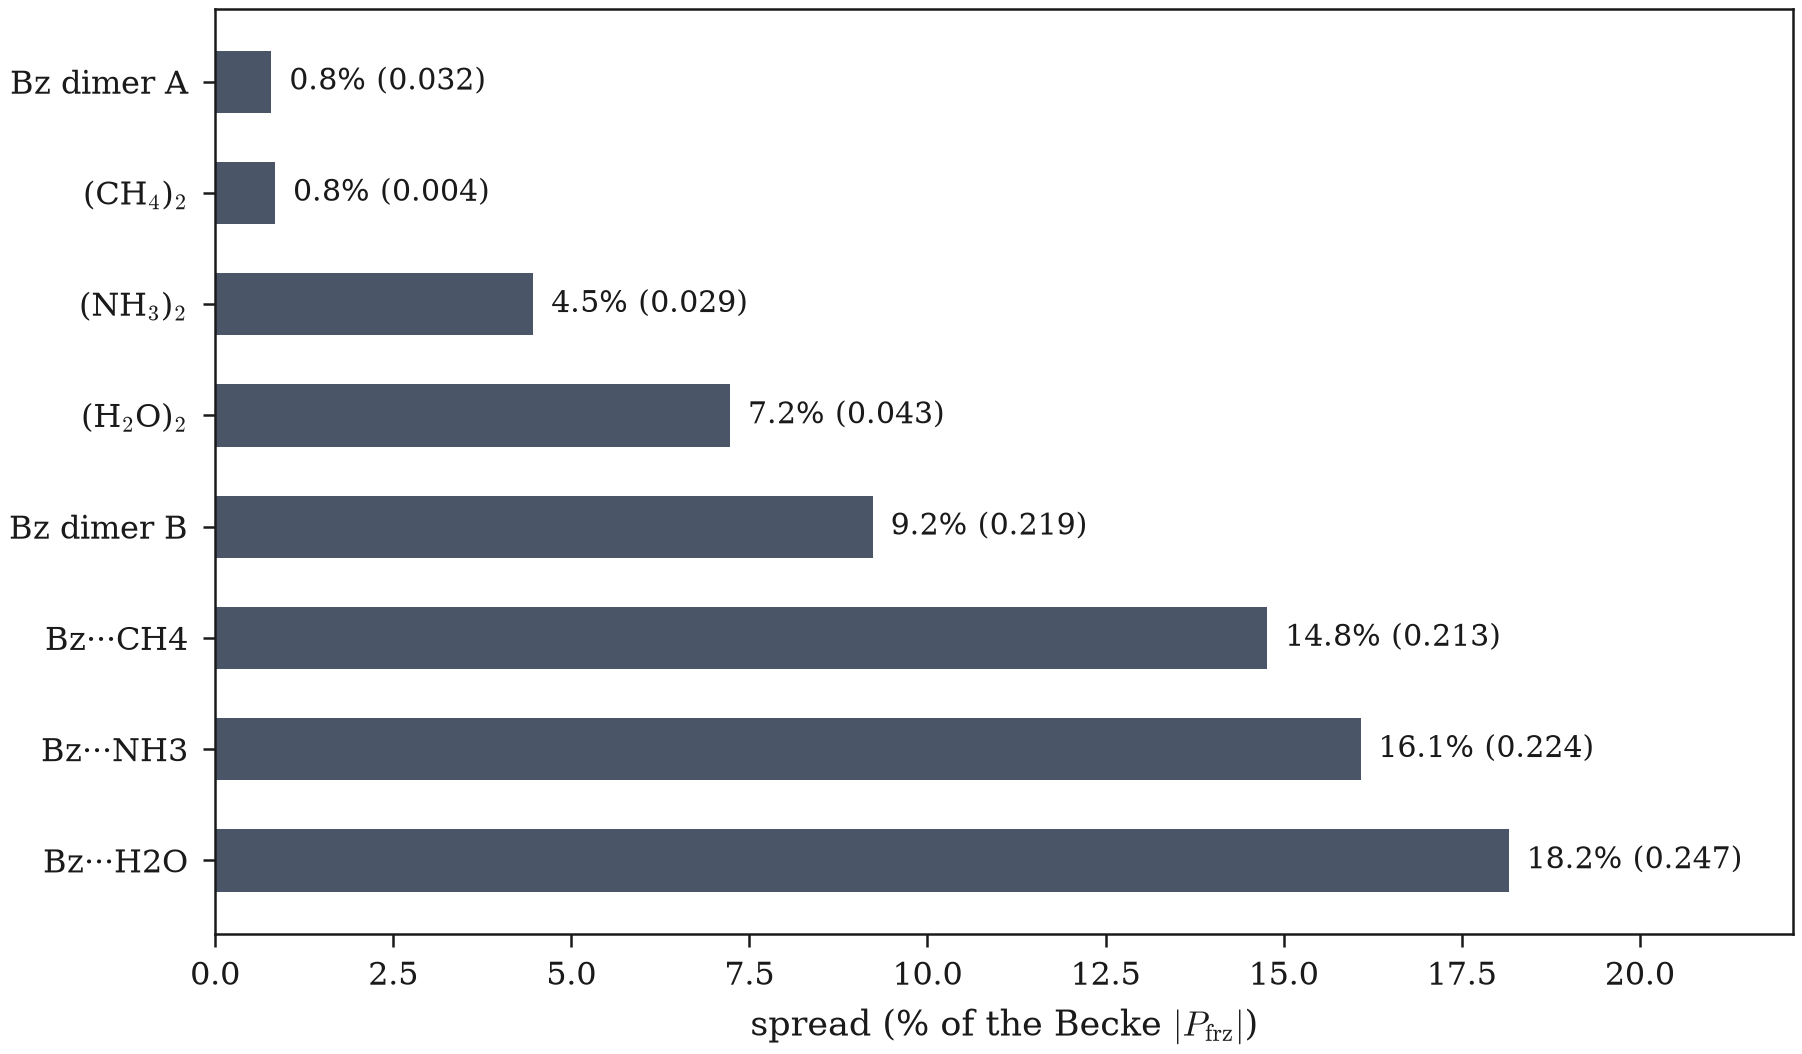
\includegraphics[width=0.92\textwidth]{figs/fig2_scheme_sensitivity.png}
\caption{\textbf{Figure 2.} How much of the reported pair term is a choice about where grid points belong: the spread of P\_frz over the four partition schemes of section 2.3, divided by the Becke-scheme value, per system, sorted. The two geometries of the same 24-atom benzene dimer sit at 0.8\% and 9.2\% and benzene...water at 18.2\%, so the percentage is a property of the arrangement rather than of the pair of molecules and cannot be collapsed into one blanket error bar. Data as in Figure 1 \prov{S2}.}
\label{fig:2}
\end{figure}

Two observations follow. First, the relative span has no pattern by interaction type: hydrogen bonding spans 7.2\% (water) and 4.5\% (ammonia), dispersion-driven complexes span 0.8\% (methane) and 18.2\% (benzene...water), and the two benzene dimer geometries differ by a factor of eleven. A single blanket uncertainty percentage for this class of method would misstate the methane dimer by more than twenty-fold. Error bars must be reported per system (Fig.\textasciitilde{}\ref{fig:2}). Second, the span is an attribution property rather than a one-particle-basis property. On the constructed water-dimer geometry, re-running the four schemes at level 1 across five basis sets gives spans of 0.0249 (STO-3G), 0.0400 (6-31G\*), 0.0382 (aug-cc-pVDZ), 0.0390 (def2-SVP) and 0.0398 (def2-TZVP) kcal/mol while P\_frz itself moves from -0.386 (STO-3G) to -0.554 (aug-cc-pVDZ) \prov{S12}: the quantity of interest drifts by 0.17 kcal/mol across the basis ladder while the scheme spread stays within $\pm$5\% of 0.039 for the four basis sets beyond the minimal one, at 0.025 in STO-3G. No better basis set will remove it, which is why it - and not grid convergence, which is 0.0081 kcal/mol over level 0 to 2 at 6-31G\* and 0.0002 over level 1 to 2 \prov{S13} - is the error bar this method has to carry.

\subsection{3.5 A limit of fragment-resolved quantities}

Because beta is a constant and the integral of rho is the electron number, the local term attributed to a fragment is exactly beta*N\_A where N\_A is its Becke population, and beta = 3.0415 kcal/mol per electron. Any scheme-induced spread in the population is therefore amplified into the fragment-resolved local term by that factor as an identity, not an estimate: for the water dimer at grid level 3 the four schemes give fragment-A populations of 10.1559 (Becke), 10.1537 (Stratmann), 10.0979 (Becke--Treutler) and 10.0478 (Becke--Rad) electrons on the official S22 geometry, a spread of 0.108 electrons which is 0.329 kcal/mol; on the constructed geometry the same spread is 0.0987 electrons, i.e. 0.300 kcal/mol \prov{S20}. Two consequences deserve stating explicitly. In a superposition difference the term cancels identically --- electron number is conserved --- so every dE\_NLC value in this paper is free of it. But any table reporting \emph{absolute} fragment energies inherits an uncertainty of this size from a quantity (atomic population) that the method does not control. This is a property of Becke partitioning that every EDA scheme shares, and we state it rather than claim it as a contribution.

A related implementation note: attributing the local term softly, by evaluating all fragment factors s\_A at every grid point rather than assigning each point to one owner, changes these numbers by at most 8.7e-7 electrons (2.6e-6 kcal/mol after multiplication by beta). The soft and hard readings of the local term are numerically the same thing, which is worth recording because the two are sometimes discussed as if they competed.

\section{4. Limitations}

\textbf{This is not an energy decomposition analysis.} We split dE\_xc into the nonlocal term and everything else, and we resolve the nonlocal term into fragment pairs. We do not separate electrostatics, exchange-repulsion, polarisation or charge transfer, and the resulting components are therefore not comparable term-by-term with ALMO-EDA or SAPT(DFT) output. Counterpoise-corrected interaction energies are reported in section 3.2 for six of the eight systems, but dE\_NLC itself needs no such correction: it is evaluated at fixed (non-self-consistent) superposed density, so basis-set flexisation does not enter it, which is precisely why it converges a grid level earlier than dE\_int does \prov{S10}.

\textbf{The nonlocal term is not the dispersion energy.} Section 3.2 is the evidence: dE\_NLC accounts for anywhere between 16\% and 97\% of dE\_xc across the seven complexes where that share is defined by our own cancellation test (Fig.\textasciitilde{}\ref{fig:1}) - and note that this is not a smooth ladder: the two geometries of the same benzene dimer give 97\% and 52\%. The eighth complex, the methane dimer, is the case a percentage cannot describe at all: its two parts carry opposite signs, so the nonlocal term is not a fraction of the change but the thing that has to overcome it. A quantity whose relation to another varies that far - and in one case changes character - cannot be identified with it. We use "dispersion" only when quoting external work, and the values in Table 1 should be read as "the contribution of the VV10 term", not as a dispersion energy.

\textbf{Cross-program check: ORCA 6.0.1 agrees on the reported quantity, on all eight systems.} Our explicit sum had only ever been checked against PySCF's native kernel, and both live in one library, so they could share an error in the functional parameters or in the kernel convention. That check now exists against a second program, and on more than the two systems we first reported. ORCA 6.0.1 prints the term natively for \texttt{! WB97X-V} as \texttt{NL Energy, E(C,NL)}; the control showing that the label is VV10-specific rather than a generic DFT printout is \texttt{evidence/orca\_control/h2o\_wb97x.out}, an $\omega$B97X run with no \texttt{-V}, which contains no such line \prov{S18}. Twenty-four serial runs - the water dimer and benzene sandwich (S22 \#2, \#11) on the cluster, the other six systems on this machine, all at S22 official complex geometries with 6-31G*, each terminating normally with a converged SCF and carrying exactly one \texttt{NL Energy} line - give, for the superposition difference that Table 1 reports. The last two columns compare the residual with the partition-scheme span of the same row (\S{}3.4), which is the quantity a referee has to be smaller than to be informative:

\begin{table}[htbp]
\centering
\begin{tabular}{llllll}
\toprule
\textbf{system} & \textbf{$\Delta$E\_NLC ORCA} & \textbf{$\Delta$E\_NLC PySCF} & \textbf{difference} & \textbf{span} & \textbf{residual/span} \\ \midrule
water dimer (S22 \#2) & -0.5931 & -0.5935 & 0.0004 (0.07\%) & 0.0435 & 0.009 \\
ammonia dimer (S22 \#1) & -0.6745 & -0.6780 & 0.0035 (0.51\%) & 0.0290 & 0.120 \\
methane dimer (S22 \#8) & -0.5160 & -0.5170 & 0.0010 (0.19\%) & 0.0040 & 0.242 \\
benzene...water (S22 \#17) & -1.2522 & -1.2590 & 0.0068 (0.54\%) & 0.2470 & 0.028 \\
benzene...ammonia (S22 \#18) & -1.3189 & -1.3270 & 0.0081 (0.61\%) & 0.2240 & 0.036 \\
benzene...methane (S22 \#10) & -1.3912 & -1.4040 & 0.0128 (0.91\%) & 0.2130 & 0.060 \\
benzene dimer B (S22 \#20) & -2.3685 & -2.3880 & 0.0195 (0.82\%) & 0.2189 & 0.089 \\
benzene dimer A (S22 \#11) & -4.3252 & -4.3668 & 0.0416 (0.95\%) & 0.0320 & \textbf{1.301} \\
\bottomrule
\end{tabular}
\end{table}

All eight agree to better than 1\% of the term, and the residual tracks the magnitude of $\Delta$E\_NLC rather than the size of the system, which is what a quadrature difference looks like. Three things must be said about it rather than glossed. First, the grids are not matched - ORCA uses its own nonlocal quadrature (Lebedev-110, IntAcc 4.004) against PySCF's \texttt{grids.level=1} - so the residual is the joint grid-plus-implementation difference and we do not attribute it to either side. Second, in seven of the eight systems the cross-program residual is smaller than the attribution span it would have to resolve, by 8 to 100 times; the exception is the benzene sandwich, where 0.042 kcal/mol is 1.3x the 0.032 kcal/mol span for that same geometry. That single row is the warning this comparison exists to provide: cross-program noise can be of the same order as the quantity being resolved, so it must never be folded into the attribution uncertainty. Third, the two water monomers of S22 \#2 are not equivalent (donor r\_OH 0.9639/0.9571 vs acceptor 0.9590/0.9590), so the monomer term had to be computed twice - using 2x one monomer would have introduced \textasciitilde{}0.0004 kcal/mol, exactly the size of the residual. A repeat of one input inside the same allocation reproduced its VV10 term to 1.6e-11 Eh, so the residual is not run-to-run noise \prov{S18}. The widened set was assembled after an audit of our own record found that \texttt{evidence/orca\_widen/orca\_widen.json} marked all twelve of its first runs \texttt{converged: false} while the archived outputs print \texttt{SCF CONVERGED AFTER n CYCLES} and \texttt{ORCA TERMINATED NORMALLY}: the flag came from a criterion that looked for a different program's wording. The flags were re-derived from the logs without re-running anything, with the assertion that no energy value moves (\texttt{evidence/orca\_widen/generator\_rescan\_convergence.py}), and the table above is generated from the tracked artefacts by \texttt{evidence/orca\_widen/generator\_cross\_program\_table.py}, which refuses to emit it if the system list disagrees with the one it declares, or if any row's basis, grid level or counterpoise setting disagrees. One operational note belongs with the row it affects: the 24-atom parallel-displaced benzene dimer (S22 \#20) is the only run that needed four times the per-process memory allowance (\%maxcore 4000 against 1000), which changes what ORCA can hold in core and nothing about the numerical parameters; at 1000 it died in the SCF with \texttt{CANNOT OPEN FILE dimer.opot2.tmp}, and that difference is recorded on the run rather than left for a reader to rediscover.

What this also checks is the absolute value, not just the difference. An earlier log of ours recorded a \textasciitilde{}0.14 kcal/mol disagreement on the water monomer between our explicit sum and the native kernel, and we flagged the absolute fragment energies as unrefereed. That flag is now retired: the archived level-2 run gives a water-dimer nonlocal term of +52.9345 kcal/mol against ORCA's +0.084358235 Eh = +52.9356, and monomers +26.7635/+26.7644 against ORCA's +26.7646/+26.7641 - agreement at the 1e-3 kcal/mol level on the absolute quantity as well [S8, S18]. We have not re-established what that 0.14 was: the most likely cause is a comparison made before the beta$\cdot$$\int$rho counterterm was added back - \texttt{step\_f\_dispersion.terms} now adds it before reporting, and the comment at that call site exists precisely because of this confusion - but we are stating the present agreement, not a diagnosis of the old number, so the section 3.5 identity is covered by this anchor without needing that story to be true.

\textbf{How we know the literature search means anything.} The zeros in section 1 are only as good as the instrument, so we calibrated it in the same session: a known paper title was retrieved exactly (1 record), a broad concept query returned 3,317 records, and a topical AND query in the same vocabulary returned 33. By contrast the two open indexes we tried first failed the same test - OpenAlex and Crossref each retrieved a known title 4/4 times when queried by title but missed that same known, on-topic paper for 2 of 3 and 3 of 3 legitimate topical phrasings respectively. We therefore report hit counts only from the instrument that passed. Its enumeration is complete rather than sampled, and that took a second round: the result-page UI virtualises its list and gave us one record per list, and the first attempt at working around it by excluding already-read titles backfired - the title we excluded was the truncated form of the very record we were chasing (FDE-vdW's full title begins "Exact kinetic energy enables..."), so we had removed our own nearest neighbour. Going to the record endpoint instead returned every record of every list. One further trap there is worth naming, because it fails silently: that endpoint streams records in batches of 20, and a parser that overwrites rather than appends reports the tail batch as the whole result set - on a 33-record query that reads as 13, and nothing in the response says so. We now assert \texttt{len(records) == RecordsFound} on every query.

\textbf{The attribution uncertainty is intrinsic and per-system.} The 0.004-0.247 kcal/mol spread of section 3.4 does not shrink with a finer grid or a larger basis; it is a property of how grid points are assigned to atoms. Any number produced by this method carries it, and reporting a single percentage for the whole method would be wrong by more than twenty-fold for individual systems.

\textbf{Absolute fragment energies inherit a population uncertainty.} As shown in section 3.5, the local term of a fragment is exactly beta*N\_A, so the 0.108-electron spread of the attributed population over the four schemes is a 0.329 kcal/mol spread in the reported fragment energy - larger than the scheme spread of the pair term itself for the water dimer. Differences are safe; absolutes are not, unless the population convention is stated alongside them.

\textbf{Cost, and what it buys.} The explicit double sum is quadratic in the number of retained grid points; we have not implemented a sub-quadratic approximation, and the point-value kernel that PySCF ships is both cheaper and accurate to \textasciitilde{}1e-8 Ha on its own grid (section 3.1). The cost is not prohibitive in itself - JuNoLo ran the same N$^{2}$ sum over massively parallel hardware for surface calculations \prov{S14} - but it is a real constraint, and it is worth naming the trade honestly. We are therefore not claiming that this method computes dE\_NLC better. What it buys is the (i, j) index structure: the 0.92-1.08 frozen-density result of section 3.3, and the per-pair numbers behind Table 1, are not recoverable from a scheme that collapses the pair sum to point values first.

\textbf{Scope of functionals.} Everything here is the VV10 kernel with the (b, C) parameters PySCF reports for omegaB97X-V, using the same-centre pairing convention of section 2.1. Functionals whose nonlocal term uses the regularised rVV10 form have not been tested and may not share the pairing convention.

\section{5. Code availability}

The package \texttt{nlcsplit} (Apache-2.0, containing no GAMESS source) implements the kernel, the four attribution schemes, the fragment decomposition and every table in this paper; each table is produced by exactly one \texttt{step\_*.py} script whose stdout is archived under a UTC-stamped filename. Fragment boundaries come from covalent connectivity rather than hand-written atom lists, and both the geometry constructors and the official-geometry loader assert internal coordinates at construction time - three of the bugs this measure was added to catch are described in the supplementary notes. Grid, basis and scheme sensitivity are separate functions (\texttt{step2\_convergence.py}, \texttt{step\_g\_basis.py}, \texttt{step\_h\_s22.py}) rather than one combined uncertainty, and \texttt{partition\_factors()} verifies its own output against PySCF's partition weights before returning it.

\section{6. Conclusions}

We have shown that the VV10 nonlocal-correlation energy can be resolved into fragment pairs without giving up the total: the double sum is evaluated explicitly, the local part cancels identically from any superposition difference because it is exactly beta times the electron number, and the resulting blocks reproduce the total to machine precision while carrying an (i, j) index that the point-value evaluation discards.

Three things follow from applying it to eight S22 complexes at official geometries. The VV10 term is not a fixed share of the exchange-correlation contribution - 16\% for the water dimer, 223\% for the methane dimer, 97\% and 52\% for two geometries of the same benzene dimer - so reporting it as "the dispersion energy" is unsafe even within one benchmark set. The association-time change is almost entirely inter-fragment: the frozen-density pair term accounts for 0.92-1.08 of the superposition difference in the six systems checked against a counterpoise reference, with relaxation a small correction of either sign rather than an additive channel. And the dominant uncertainty is the attribution scheme, not the numerics: 0.004-0.247 kcal/mol absolute, 0.8-18.2\% relative, stable to within $\pm$5\% across the four basis sets beyond STO-3G and to within 0.001 kcal/mol between grid levels 1 and 2, with no pattern by interaction type that would let a single percentage be quoted.

What the method does not do is equally important, and we would rather the reader learn it here than in a review. It is not an EDA: it does not separate electrostatics, exchange-repulsion, polarisation or charge transfer. It is not faster than the production kernels it could be compared against - it is quadratic in the grid. Its arithmetic was for most of this project verified only against a second implementation of the same kernel inside the same library; that gap is now closed for the quantity Table 1 reports, by twenty-four ORCA 6.0.1 single points covering all eight systems, every residual below 1\% of the term (0.0004 kcal/mol on the water dimer up to 0.0416 on the benzene sandwich). An earlier version of this draft claimed such an anchor and had to withdraw it; what actually failed was not the check but our ability to find its number, because we searched for the words "nonlocal" and "VV10" in an output file that labels the quantity \texttt{NL Energy, E(C,NL)}. One scoping limit remains: the absolute value, not only the difference, is checked on the water dimer and on both of its monomers (\S{}4, where the earlier "unrefereed" flag is retired); on the other seven systems the second program checks the difference, which is what every claim in this paper is made of, and not each absolute fragment value.

Two further items are open and stated as such rather than smoothed over. The first is a number, not a missing run: re-running benzene-methane at level 2 with counterpoise on two PySCF releases reproduced every attributed quantity to within 5e-4 kcal/mol - the rounding half-step of the three-decimal printout on one side, the largest measured difference being 4.2e-4 on the pair term - but reproduced the counterpoise interaction energy only to 0.139 kcal/mol (section 2), so a counterpoise denominator is not portable between versions while the pair term appears to be. The second is a scope limit: the basis-set ladder of section 3.4 was run before the water-dimer geometry fix, and although its level-1 column agrees with the post-fix recompute to four decimals for every base the two runs share, the full ladder has not been re-run on the relaxed geometry. Separately, the literature search covers one index - Web of Science Core Collection - because Scopus was measured as unsubscribed at our institution and Embase and SciFinder were not searched at all. Within that one index, though, the search is now a full enumeration rather than a sample: every record returned by every query was read, which changed the conclusion in one place worth reporting, since a keyword-shaped novelty query is narrower than the claim it is meant to test. Six queries in the first round covered the decomposition vocabulary and found nothing in the interpretive line; adding the broadest topical query available (vdW-DF x "nonlocal correlation", 33 records, every title read) surfaced Hyldgaard, Berland and Schröder's xc-hole interpretation of the same energy \prov{S17}, which no query containing decompose, partition, fragment or pair would ever have returned. The open indexes tried instead (OpenAlex, Crossref, Semantic Scholar, arXiv) are recorded as supplementary and not as a second formal search, because their reachability was uneven and measured: OpenAlex's search route returned 21 usable responses against 14 rate-limited and 10 server-error attempts, Semantic Scholar's search route was rate-limited throughout so its keyword dimension was never actually queried, arXiv failed known-item calibration (its own abstract field contains a term that its search does not retrieve) so its zeros are not read as absence, and Scopus returned 401/403. Crossref and OpenAlex retrieve known titles reliably but miss a known on-topic paper when asked topically (section 4). The round still changed this paper: the nearest neighbour, and the reason the claim is narrower than it was written, came from it rather than from the formal search.

The package is released under Apache-2.0 with no GAMESS source in it, every number in this paper is produced by a named script whose archived stdout is part of the repository, and the two structural guards we added after finding bugs in our own geometry builders - coordinate assertions at construction time, and \texttt{partition\_factors()} verifying its own output against PySCF's partition weights before returning - are the part of this work we would most recommend copying.

\section{Appendix: provenance of every quoted number}

Each tag used above resolves to a file in this repository. "line N" means the value can be read literally at that line of the archived standard output; those stdout files are tracked, hash-listed under \texttt{evidence/*/MANIFEST.sha256}, and were not re-typed by hand.

\begin{table}[htbp]
\centering
\footnotesize
\begin{tabularx}{\textwidth}{lXX}
\toprule
\textbf{Tag} & \textbf{Artefact} & \textbf{What it fixes} \\ \midrule
S1 & \texttt{RESEARCH-20260929-lit.md} \S{}1, \S{}6 & first-round WoS/Scopus search record: strings, hit counts, search date \\
S2 & \texttt{MAIN-skeleton.md} tables 2 and 4b; \texttt{nlcsplit/logs/step\_h.json} & the level-1 S22-subset table, incl. the 0.8\% / 18.2\% nonlocal fractions \\
S3 & \texttt{nlcsplit/step\_f\_dispersion.py} & the level-1 dispersion-scale check that leaves the double sum as the only unaccounted term \\
S4 & \texttt{MAIN-skeleton.md} table 4b & the 52\%-97\% range of the same quantity across partitions \\
S5 & \texttt{nlcsplit/step\_e\_kernel.py} & explicit pair sum vs PySCF's native VV10 kernel on a fixed grid \\
S6 & \texttt{evidence/centos/20260928T165857Z\_centos-step\_c.out} line 19 & relaxed O-O = 2.901 A \\
S7 & \texttt{nlcsplit/step\_d\_floor.py}, \texttt{nlcsplit/tests/test\_kernel.py} & the local term is beta x electron number, so it cancels in any superposition difference \\
S8 & \texttt{nlcsplit/logs/step\_h.json}, \texttt{nlcsplit/logs/step\_h\_l2cp.json}, \texttt{evidence/l2cp/20260929T051912Z\_centos-l2\_benzmeth\_cp.out}, \texttt{evidence/l2cp/20260929T051849Z\_l2\_benzmeth-wsl.out}, \texttt{evidence/centos/20260928T165857Z\_centos-step\_f\_h2o2.out}, \texttt{evidence/recompute/20260929T010500Z\_step1\_geomfix.out} & cross-version pair (PySCF 2.12.1 vs 2.14.0) and the 19936 vs 20248 partitioned grid counts \\
S9 & \texttt{nlcsplit/step\_i\_gridrepr.py}, \texttt{evidence/recompute/20260929T\_step\_i\_gridrepr.out} & the two discrepancies that were previously reported as one number \\
S10 & \texttt{evidence/l2cp/20260928T213839Z\_centos-step\_h\_l2cp.out}, \texttt{evidence/l2cp/20260929T051912Z\_centos-l2\_benzmeth\_cp.out}, \texttt{nlcsplit/logs/step\_h\_l2cp.json} & level-2 with counterpoise, all six S22 subsystems complete, including the \texttt{p\_over\_ds} column behind the 0.92-1.08 ratio \\
S11 & \texttt{RESEARCH-20260929-lit.md} \S{}6.2-6.3 & published comparison value for JCTC 3c00903 (full text via ChemRxiv green OA 10.26434/chemrxiv-2023-nc64t) \\
S12 & \texttt{evidence/recompute/20260929T003144Z\_stepg-recompute.out}, cross-checked against \texttt{evidence/centos/20260928T165857Z\_centos-step2.out} & five-basis ladder of P\_frz and of the four-scheme span at level 1 on the constructed water-dimer geometry; its level-1 column agrees with the earlier CentOS run to four decimals for the three bases both runs share \\
S13 & \texttt{evidence/centos/20260928T165857Z\_centos-step2.out} lines 17-20, per-level values at lines 2-15 & cross-grid spread per basis (sto-3g 0.0010, 6-31G* 0.0081, aug-cc-pVDZ 0.0067); the 0.0002 for 6-31G\* over level 1 to 2 is the difference of lines 8 and 9 \\
S14 & Lazić, Atodiresei, Alaei, Caciuc, Blügel and Brako, \emph{Comput. Phys. Commun.} \textbf{181}, 371-379 (2010), DOI 10.1016/j.cpc.2009.09.016; open preprint arXiv:0810.2273v1; judgement in \texttt{RESEARCH-20260929-lit.md} \S{}10 & the closest published decomposition of a nonlocal term, read in full text \\
S15 & \texttt{evidence/retrieval\_calibration/oa\_stab.js}, \texttt{evidence/retrieval\_calibration/openalex\_stability.json}, \texttt{evidence/retrieval\_calibration/xref\_calib2.js}, \texttt{evidence/retrieval\_calibration/xref\_r3.js} & measured recall of the open indexes: 4/4 known titles at rank 0, 0/4 and 1/3 for legitimate topical strings \\
S16 & \texttt{RESEARCH-20260929-lit.md} \S{}8.1 & the institutional-access precondition of the search, and why the first round was counted from the UI \\
S17 & \texttt{RESEARCH-20260929-lit.md} \S{}13 & second round: full enumeration through WoS's own record endpoint (RecordsSearched = 58,664,816, search date 2026-09-29), the three calibration strings reproduced record-for-record, the two zero-hit strings, complete readings of the two 4-record and four broad strings, and the three added citations whose DOIs were checked against both Crossref and WoS \\
S18 & \texttt{nlcsplit/logs/orca\_anchor.json}, \texttt{evidence/orca\_run/h2o\_dimer.out}, \texttt{evidence/orca\_run/h2o\_mono0.out}, \texttt{evidence/orca\_run/h2o\_mono1.out}, \texttt{evidence/orca\_run/benz\_dimer.out}, \texttt{evidence/orca\_run/benz\_mono0.out}, \texttt{evidence/orca\_run/benz\_mono1.out}, \texttt{evidence/orca\_run/MANIFEST.sha256}, \texttt{evidence/orca\_control/h2o\_wb97x.out}, \texttt{evidence/orca\_control/h2o\_wb97xv.out}, \texttt{evidence/orca\_control/MANIFEST.sha256}, \texttt{evidence/orca\_widen/orca\_widen.json}, \texttt{evidence/orca\_widen/RECHECK\_convergence.txt}, \texttt{evidence/orca\_widen/generator\_rescan\_convergence.py}, \texttt{evidence/orca\_widen/generator\_merge\_run.py}, \texttt{evidence/orca\_widen/generator\_cross\_program\_table.py}, \texttt{evidence/orca\_widen/cross\_program\_table.txt}, \texttt{evidence/orca\_widen/MANIFEST.sha256} & the cross-program referee: three ORCA 6.0.1 runs each (S22 official geometries, 6-31G\*, every run with a converged SCF and exactly one \texttt{NL Energy, E(C,NL)} line) --- six for water and the benzene sandwich from \texttt{nlcsplit/logs/orca\_anchor.json}, eighteen more archived under \texttt{evidence/orca\_widen/} (one log per run, each listed with its sha256 in \texttt{evidence/orca\_widen/MANIFEST.sha256}) covering ammonia, methane, benzene...water, benzene...ammonia, benzene...methane and the parallel-displaced benzene dimer; the per-file sha256 manifests; the omegaB97X (no \texttt{-V}) control that prints no such line; the re-scan that corrected twelve falsely-flagged \texttt{converged} fields without touching any energy; and the generator that emits the eight-row comparison and refuses if the system list disagrees with the one it declares, or if any row's basis, grid level or counterpoise setting disagrees \\
S19 & \texttt{evidence/centos/20260928T165857Z\_centos-step\_c.out} lines 6, 15 and 24 & the level-0 ratios of the inter-fragment pair term to the superposition difference: 1.017 for the water dimer at the official S22 geometry, 1.025 at its omegaB97X-V-optimised geometry, and 0.915 for the benzene sandwich - the third of these is a different system, which is why it is not folded into the 0.92-1.08 band \\
S20 & \texttt{nlcsplit/step\_k\_population.py}, \texttt{evidence/population/20260929T131530Z\_stepk\_pop-official.out}, \texttt{evidence/population/20260929T131055Z\_stepk\_pop-constructed.out} & the level-3 four-scheme population table for the water dimer, from which beta*N\_A is read; both runs assert that the fragment populations sum to the electron number. Re-running them is also what showed that the earlier tabulation of this number in the work log was labelled "official geometry" but reproduces only on the constructed one \\
S21 & \texttt{evidence/agentb\_sweep/20260928T071951Z\_agentb-sweep\_631gstar.txt}, \texttt{evidence/agentb\_sweep/20260929T151414Z\_step\_l\_sweep\_compare\_levels0-9.out}, \texttt{evidence/agentb\_sweep/20260929T151414Z\_step\_l\_sweep\_compare\_levels0-9.json}, \texttt{nlcsplit/step\_l\_sweep\_compare.py} & the independent sweep (water-monomer nonlocal term at levels 0-9, self-consistent and again on one fixed density matrix, ending in a partial \texttt{atom\_grid} scan that dies on an unsupported angular grid), and the archived stdout plus sidecar JSON of our comparison against it, which carry the per-level difference column behind section 2.1 - the sweep file alone has no comparison column. Produced by the shipped script; its level-9 sum covers 9.2e10 point pairs over 428,920 kept grid points, which is why that one row took hours. The \texttt{levels0-8} snapshot taken mid-run is kept beside it, hashed, as the record of what was known before level 9 landed; its header announces the intended 0-9 range, which is why that filename says 0-8 and this one says 0-9. \\
\bottomrule
\end{tabularx}
\end{table}

Three absences are stated rather than hidden. \texttt{evidence/centos/...step\_f\_h2o2.out} predates the water-dimer geometry fix (its inter-fragment minimum is 2.0258 A against 1.95 A in \texttt{evidence/l2cp/}), so S8 cites it only for the component accounting, never as a current-geometry result. S15's files were sitting in \texttt{scratch/}, which is gitignored - they were promoted into \texttt{evidence/} on 2026-09-29 for exactly that reason. And one distinction has to be kept: S6 and S13 come from the same CentOS batch timestamped 2026-09-28T16:58, which is earlier than the geometry fix, while S12's primary artefact is a recompute run afterwards. Within that earlier batch the initial S22 structure and the relaxed one are distinguishable (the level-0 6-31G* value -0.5316 appears in S13's ladder, while the -0.5975 of the relaxed structure does not), so S13's cross-grid spreads are read here as measured on the \emph{initial} S22 geometry, not on the relaxed one that carries the headline numbers. The level-1 column of that same ladder agrees with the later recompute to four decimals for all three bases the two runs share, so the grid-convergence conclusion does not turn on which geometry was used - but that was checked after the fact, and re-running the full ladder on the relaxed geometry stays an open task rather than a claim.
\bibliographystyle{unsrtnat}
\bibliography{references}
\end{document}
